\documentclass{article}

\usepackage[margin=1in]{geometry}
\usepackage[T1]{fontenc}
\usepackage[fontsize=12pt]{fontsize}
\usepackage{fancyhdr}
\usepackage{extramarks}
\usepackage{amsmath}
\usepackage{amsthm}
\usepackage{amsfonts}
\usepackage{tikz}
\usepackage[plain]{algorithm}
\usepackage{algpseudocode}
\usepackage{multicol}

\usetikzlibrary{automata,positioning}

\linespread{1}

\pagestyle{fancy}
\lhead{\hmwkAuthorName}
\chead{\hmwkClass: \ \paprTitle}
\rhead{\today}
\lfoot{\hmwkTitle}
\cfoot{\thepage}

\renewcommand\headrulewidth{0.25pt}
\renewcommand\footrulewidth{0.25pt}

\setlength\columnseprule{.25pt}
\setlength{\columnsep}{2.5pc}
\setcounter{secnumdepth}{0}


\newcommand{\hmwkTitle}{Paper Summary\ \#1}
\newcommand{\paprTitle}{\\ An integrated model of ERP success}
\newcommand{\hmwkDueDate}{May 9, 2023 @ 23:59, EST}
\newcommand{\hmwkClass}{CIS 562 - Enterprise Architecture}
\newcommand{\hmwkAuthorName}{\textbf{Cason Konzer}}


\title{
    \vspace{2in}
    \textmd{\textbf{\hmwkClass:\ \\ \hmwkTitle}}\\
    \normalsize\vspace{0.1in}\small{Due\ on\ \hmwkDueDate}\\
    \vspace{0.1in}\Large{\textit{\paprTitle: the critical role of task-context alignment}}
    \vspace{3in}
}

\author{\hmwkAuthorName}
\date{\today}

\begin{document}

\maketitle

\pagebreak

\tableofcontents
\listoffigures
\newpage

\section{Summary}
In this paper summary we will be taking a condensed look at Gavidia, Junglas, and Chou's recent publication ``An integrated model of ERP success: the critical role of task-context alignment'' \cite{integrated_erp}.
ERP (Enterprise Resource Planning) systems centralize data availability, with goals of increasing business efficiency.  
Under such a system, differentiated business units have the ability to work in a single application, easing access to cross functional insights. 

Implementations of an ERP can be complex, risky, and costly. 
Measuring the increase in business efficiency, or ROI (Return on Investment), is hard to do in practice as a long term analysis is needed and a plethora of confounding variables exist. 
\cite{integrated_erp} looks to model the success of ERP Implementations by their driving factors, specifically with respect to business context. 

\subsection{Research Question \& Reasoning}
The general scope of the paper looks to address the success of ERP implementation from an organization context perspective. 
In doing so the authors look to identify decisions in the implementation process which influence the chosen ERP solution and its benefits to the business. 
From this we can formulate the following research question at hand; \emph{How do contextual organization factors drive key implementation decisions effecting the final success of an ERP system in business performance}? 

In choosing such a question, the authors build upon their analysis of prior literature. 
They found the list of CSFs (Critical Success Factors) to be ever expanding with a general lack of consensus on definition. 
Often studied were core project management and technical implementation factors, with contextual factors receiving less attention. 
Granted, the authors' study is not novel in the area of contextual factors, but due to the lack of empirical data, communal consensus, and relevance to the `real world,' further study was needed. 

Driving the study of ERP systems and their implementation is at core ERP system necessity in business today. 
From small businesses to fortune 500 enterprises, ERP systems support daily tasks from operations in accounting and resource planning to forward looking strategic decisions for the leaders in the organization. 
In this manner the study of ERP system integration is vital to future adoption by and success of new businesses. 

\subsection{Hypothesis}
The hypothesis proposed by the authors is that while common management and technical factors effect ERP implementation success, the most important factors are those which bridge management decisions with operational tasks. 
Inherently this bridging ensures that the management brings about an ERP implementation which meets the needs of the end users. 

While the metrics used by management for strategic decisions are often common across organizations, the input data varies based on context. 
One may consider these differences in the context of business products, for instance an e-commerce business will have a much different ERP implementation than a trade (mechanic, electrician, etc.) contracting company. 
Previously studied contextual factors included, but are not limited to: organizational size, structure, time frame, organizational readiness, resources, maturity, and psychological climate and individual behavioral characteristics \cite{integrated_erp}.
Still, contextual factors encompass much more, even outside the business, such as market competition, economic situation, legal regulation, and integrator domain expertise. 

\subsection{Methodology}
The authors find the prior literature to rely heavily upon survey studies, but identify a unsatisfactory extraction of detail from such a methodology. 
Generally speaking, survey studies are tightly structured and lack the ability to allow the interviewee to expand upon topics they deem important as one would in less structured conversation. 
Under such a realization, and with support from literature on study methods, the authors choose to conduct a case study of ERP implementations in the field. 

Building on the CSFs examined in previous works, the authors created a semi-structured interview guide aimed at facilitating unstructured conversation on business implementation of an ERP system.
A high level view of the guide consists of a company description, strategic situation, project management, software selection, implementation process, and success of the implementation \cite{integrated_erp}.
This approach was aimed to uncover the `real world' nuances of ERP implementation which had not yet been discovered via theoretical discussions. 

In selection of companies to study, the authors consulted with ERP system implementers aiming for a diverse selection of companies across contextual dimensions. 
In total three organizations were selected, all of which were located in Spain. 
Prior to the interview process background data was collected from the companies and the ERP implementation process to support the interviewer. 
Interview questions were left open to the interpretation of the interviewees, each organization had multiple, and the sessions were recorded for later analysis. 
Unclear from the authors is why the case study chose only three organizations to interview, although likely due to available funding and research timelines, or the centralized location of Spain, addressed later as a potential limiting factor to drawing conclusions. 
After the interview process, analysis was conducted to draw conceptual and thematic information, along side meta-data from the case.  

The selected organizations included a small motorsports equipment reseller, a mid-sized ship building company, and a large equipment rental corporation. 
In such a manner a variety of context was analyzed across industry, standardization, structure, multinationality, and ERP usage, among other dimensions. 

\subsection{Findings}
Starting with the smallest, sole proprietorship, motorsports business of 10 employees, the owner motivated the implementation of an ERP system. 
With plans for future growth, and as an e-commerce business, the focus of the implementation was with respect supply chain management, inventory, and financials. 
Additionally crucial to the implementation was access via mobile devices and communications functionality due to the large customer base and need for frequent travel with respect to supplier negotiations. 
In summary the motorsports business had flexibility in their implementation with little dependencies and rather general requirements. 
As a result the company chose an off the shelf solution, although failed to meet budget goals and were unhappy with the licensing fees. 

The mid-sized ship building company was family owned, consisted of 260 employees, and maintained domestic contractual projects in parallel. 
Acquiring business consistent of winning bids for project proposals on the market, given a set of design and timeline requirements. 
The critical factor of successful acquisition and profitability was a timely, accurate, and competitive bid.
In facilitating this the ERP systems required integration of specialized naval engineering software with ties to materials pricing and labor costs from historical projects. 
The project was championed by the owner, with a clear understanding of the ROI opportunity, yet a lack of support existed from line management due to low experience with ERP systems. 
The final implementation was a customized software which was built by an implementor specialized in ERP for ship building and knowledgeable of the specialized engineering softwares in use. 

The last case of the large equipment renter consisted of 25 regional corporations, employing 2000 individuals across multiple countries. 
Due to a recent merger, the company had the unique case of two legacy ERP systems in place of which they needed to bring conformity. 
Along with the typical ERP use cases, the company had specialized use cases required for equipment maintenance, in workshop and in field, in addition to fleet management and international accounting. 
The legacy systems provided extensively developed applications specific to subsidiary use cases from an operational perspective, but lacked the required conformity for global management. 
As a result, the project, championed by the general manager, kept the legacy systems and integrated them into a global facing ERP system siting atop the others. 

All of the case studies deemed the implementation to be successful and found themselves in a better position for growth, efficiency, and customer satisfaction. 
The champions all validated their implementation and decision based on their unique contextual factors \cite{integrated_erp}. 
After implementation, success was never clearly measured, but rather taken as given such that the projects' objectives were met. 

\subsection{Interpretation}
Anecdotally, the authors took the lessons learned from the cased studies to create a model for ERP implementation success. 
Their model bridges contextual factors with objectives of the ERP, of which drive the implementation decisions, execution, and success (Figure~\ref{fig:ERP_Success_Model}). 
Under this model, and as observed though the interviewing process, the contextual factors are shown to be the foundation of the implementation from a managerial perspective. 
Who will use the system and how it will be used are found to be critical to the context, objectives, and implementation. 
Execution is found to be segregated into project and technical tasks, with success to be measured in terms of the tactical and strategic outcomes. 
The authors build upon previous literature by bringing insights from industry with a more unstructured, and human, case based interview approach to information acquisition and analysis. 
Generally speaking, the authors acquired and extracted the common knowledge of ERP system implementers and consultants.

\newpage

\section{Appendix : Figures}

\begin{figure}[ht!]
    \centering
    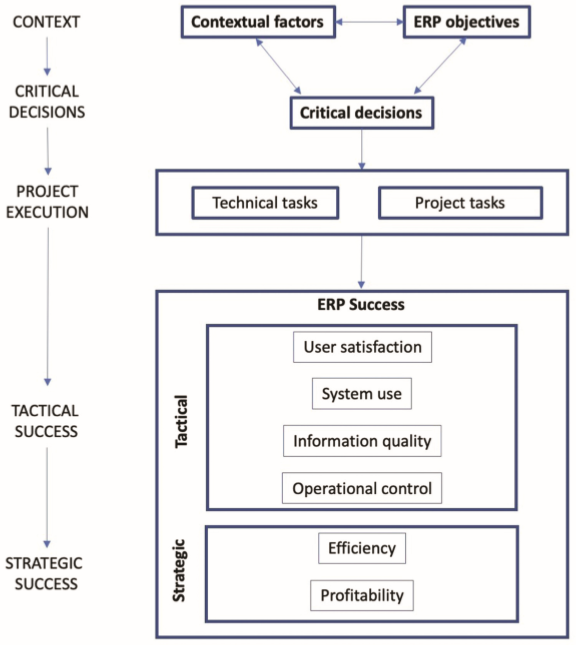
\includegraphics[width=\textwidth]{./ERP_Success_Model.PNG}
    \caption{A model of context-driven critical decisions for ERP success \cite{integrated_erp}.}
    \label{fig:ERP_Success_Model}
\end{figure}

\newpage

\bibliography{./konzer_cason_CIS_562_paper_summary_1.bib}{}
\bibliographystyle{ieeetr} % abbrv, acm, alpha, apalike, ieeetr, plain, siam, unsrt, tugboat
\end{document}